
\chapter{Related Work}

In this chapter we will give a brief overview over different services offered in the Web, to point out what services in the Web all can be.
We then introduce the \textrm{\acrlong{eca}(\acrshort{eca})} paradigm, an event-driven approach to impose reactivity.
And finally we point out existing rule languages and engines that exploit the \textrm{\acrshort{eca}} paradigm.

\section{Services in the Web}
The term service in the context of the Web is ambiguous and there have been a lot of different approaches to offer services within the Web, some of the latest used in cloud computing being \textrm{\acrlong{paas} (\acrshort{paas})}, \textrm{\acrlong{saas} (\acrshort{saas})} and \textrm{\acrlong{iaas} (\acrshort{iaas})}.
The term \textrm{\gls{webservice}} is widely understood as interfaces for communication between applications over a network, but has seen many specific adoptions.
We will point out some main research areas on service-orientation within the Web and give an idea of what kind of services in the Web we intend to orchestrate with our conceptual model.

Remote execution of programs on other computers has always been a strong research area. And with the coinage of the term \textrm{\gls{www}}~\cite{DBLP:journals/en/Berners-LeeCGP92}, there were also trends towards services offered through the Web; computers waiting in the Web for a request in order to execute some application logic and return an answer.
The encapsulation of functionality into services~\cite{peltz2003web} in order to offer them to other applications is called service-oriented architecture (\textrm{\acrshort{soa}})~\cite{perrey2003service}.
Adopting \textrm{\acrshort{soa}} internally to an application means splitting the application into smaller pieces, which then communicate via these services among each other.
This does not only provide robustness, it also allows the reuse of functionality through services.
Moreover these services can be offered to other applications and also to the Web, thus allowing others to access certain functionality or even the whole application.
All nodes in the Web are stand-alone entities, which offer services of some sort, be it a webpage, data, instant measurements or functionality.
This makes the Web itself a service-oriented architecture and all these services are naturally services in the Web.
It is for its advantages that \textrm{\acrshort{soa}} has received a great deal of attention and has been widely adopted, mostly throughout the Web.
This lead to an increasing number of Web accessible services and their compositions, the so called \textrm{\gls{mashup}s}.
An empirical study~\cite{conf/icws/HuangFT12} on a directory, which they call the \textit{"[...] most active Web APIs and mashups collection"}, and data taken from this resource (depicted in Figure \ref{fig:NumOfAPIs}) seem to underline a growing popularity, at least in terms of publishing services through this directory.

\begin{figure}[!ht]
  \centering
  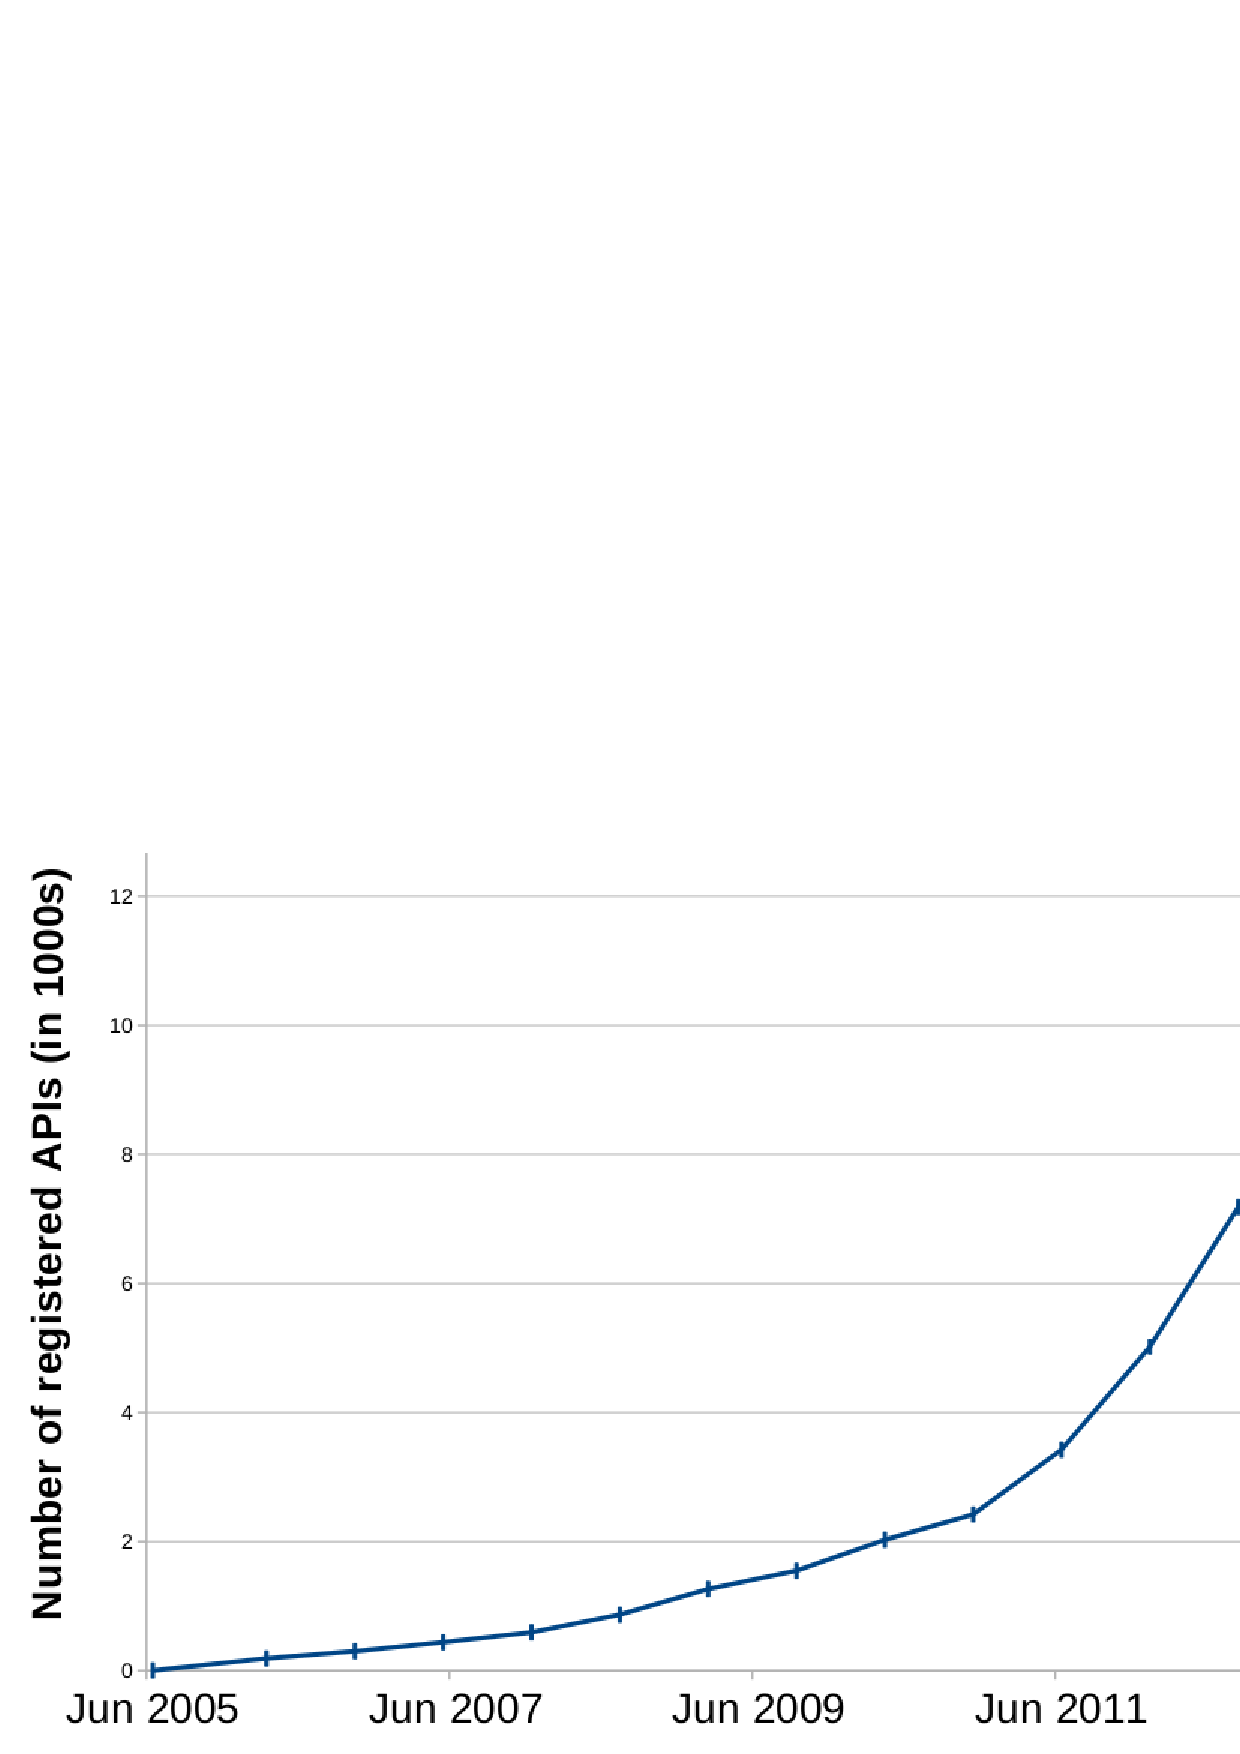
\includegraphics[width=0.55\textwidth]{figures/NumOfAPIs}
  \caption{Number of registered APIs in the ProgrammableWeb directory by date}
  \label{fig:NumOfAPIs}
\end{figure}


\subsection{Requesting Services in the Web}
An early adoption of the service concept to computers were the \textrm{\acrlong{rpc}}s (\acrshort{rpc})~\cite{Birrell:1984:IRP:2080.357392}.
Through \textrm{\acrshort{rpc}} a piece of code can be executed on a different machine, than the one which is calling the procedure.
It is basically achieved via inter-process communication and doesn't necessarily require the Web.
Even more since when \textrm{\acrshort{rpc}} was invented, the \textrm{World Wide Web} wasn't even postulated by Tim Berners-Lee. 
\textrm{\acrshort{rpc}} also found its use in grid computing~\cite{seymour2002overview} and through this, opened doors into the field of distributed computation.
The \textrm{\acrshort{rpc}} paradigm isn't bound to certain technologies and thus, has been implemented in a lot of different programming languages.
These implementations were tightly bound to the respective language that was used, which resulted in incompatibility among them.
It became necessary to enhance \textrm{\acrshort{rpc}}'s in order to get cross platform compatibility.
The abstraction of \textrm{\acrshort{rpc}} through the \textrm{\acrlong{xml}} (\textrm{\acrshort{xml}})~\cite{bray1998extensible}, which is called \textrm{\acrshort{xmlrpc}}, compatibility between services that used different technologies was easier to achieve.

Since \textrm{\acrshort{xmlrpc}} was held relatively simple but received a lot of attention, it was further enhanced.
Together with additional proposed functionality, \textrm{\acrshort{xmlrpc}} heavily influenced \textrm{\acrlong{soap}} (\textrm{\acrshort{soap}})~\cite{box2000simple}.
\textrm{\acrshort{soap}} is accompanied by the \acrlong{wsdl} (\textrm{\acrshort{wsdl}})~\cite{christensen2001web} which is used to describe the interfaces to \acrshort{soap} services.
Through \textrm{\acrshort{soap}} and \textrm{\acrshort{wsdl}} a client for the service can issue a request for the \textrm{\acrshort{wsdl}} information of the service and retrieves all interface specifications he requires in order to issue a call to the actual service.
The service specifications are then incorporated into the existing application as if it is a local function call.
\textrm{\acrshort{soap}} has found its applicability in business applications~\cite{journals/itpro/BarrosD06} and was enhanced with a lot of industrial standards, also called the "WS-*" specifications, e.g. WS-Addressing, WS-Policy or WS-Security.

\index{CORBA}
Another initiative that aimed for eased communication between different platform is the Common Object Request Broker Architecture (\textrm{CORBA})~\cite{dec1991common}.
As the name already suggest it is an object-oriented approach and it allows the exchange of whole objects.
\index{ORB}
\textrm{CORBA} relies on its communication layer, the Object Request Broker (\textrm{ORB}), which forms the basis of its architecture.
The platform-specific \textrm{ORB}'s provide the communication abstraction, which free the application from platform dependencies.
\index{IDL}
Similar to \textrm{\acrshort{soap}}'s \textrm{\acrshort{wsdl}}, \textrm{CORBA} has its Interface Definition Language (\textrm{IDL}) to provide information about the objects to be offered and accessed.
An object is instantiated by an application and the interface to this instance is offered through the \textrm{ORB}.
Another application attached to the \textrm{ORB} can then access all public variables, data structures and functions of this object.
This means not only remote access to variables and data structures, but also remote function invocation.
\textrm{CORBA} requires the implementation of object-oriented mechanisms in programming languages which aren't object-oriented.
This can be technically difficult and become an eventually tedious task.
\textrm{CORBA} allows communication between applications written in different programming languages and which are running on the same physical computer, as well as the communication between different computers in the same network.
With the Internet Inter-\textrm{ORB} Protocol (\textrm{IIOP}) it is also possible to connect \textrm{ORB}'s over the Web.
Through this, the offered objects can become services in the Web, but they are shielded by the \textrm{ORB}.


\subsection{Services in the Web become Web Resources}
\index{REST}
All the afore mentioned approaches require a specific protocol and are therefore incompatible with each other.
For this reason and its simplicity, an architectural style has gained popularity which frees application from this constraint: Representational State Transfer (\textrm{REST})~\cite{fielding2000architectural}.
\textrm{REST} concentrates on the roles of components and on constraints upon interactions between them.
An important architectural constraint is that all communication is stateless, which means for a client-server communication, no state is stored on the server.
Therefore all informations required for a single interaction need to be provided within one request.
This allows for the definition of simple and well-defined interfaces, since responses are not bound to a certain session state. 
\index{REST}
Services within the Web that adhere to the \textrm{REST} architecture are called \textrm{RESTful} Web services.
\index{URI}
\index{Web Resources}
\textrm{RESTful} Web services provide access to their data and functionality through grouped \textrm{Web Resources}, which can be identified vie Uniform Resource Identifiers (\textrm{URI}).
Simple access to services in the Web without communication overhead and required negotiation before using it, increased \textrm{REST}'s popularity and spread it into more application fields.
There is for example the upcoming concept of the \textrm{Web of Things}~\cite{Guinard2011WoT}, which aims to incorporate smart things (e.g. tagged things, sensor measurements, device controllers, etc.) into the Web through \textrm{REST} interfaces.
\textrm{REST} brings advantages into the context of smart things connected to the Web, because incompatible standards and protocols were used by different manufacturers of such things.


\subsection{Composing Services in the Web}
% \section{Weakening the Relevance of the Client-Server Model}
% \textit{Dropping the Client-Server Model}\\
% \textit{The Interweavement of Client and Server}\\
Webpages emerged into dynamic sites on the web through the upcoming of scripting languages to control the browser and the webpage itself.
With all their infrastructure in the background on the server they became literally applications.
\index{Web Application}
These Web applications (\textrm{Web Apps}) went even more responsive with the advent of asynchronous calls from the browser to the server, which allows to load data into the current webpage while the user is interacting with it.
\index{API}
\index{Web API}
Those asynchronous calls are requests to services, which act as the application programming interface \textrm{API} to the \textrm{Web App} (\textrm{Web APIs}) which sits on the server.
As a side-note, the term \textrm{Web API} not only comprises server-side interfaces but also client-sided ones (e.g. the browser), after all they are also interfaces to the Web.
For server-side \textrm{Web APIs} this means that these services can be accessed from other entities in the Web than just browsers, which eases application to application communication.
Basically a \textrm{Web App} can be controlled without the user interface, which is often delivered by the provider of the application.
Imagine not going to the Google webpage anymore to make a search and crawling through the results, but you have your own application doing it for you and processing the results instantly.
There is a trend of \textrm{Web App} providers to publish their \textrm{Web API} in order to grant easy access to it.
This lead to an increase of the number of \textrm{Web App Mashups} in the past few years.

\index{Mashup}
\textrm{Mashups} combine data and functionality of more than one service in the Web in a new site.
Simple services from different sources can be combined into more powerful ones, which can in turn again be composed and so on.
These service compositions assemble data and services in a novel way which provides a new perspective.
Ever since services were accessible in a more or less convenient way, \textrm{Mashups} have been developed as well.
On of the first Web service \textrm{Mashups}~\cite{wwwHosuingMaps}, was invented in the same year after Google Maps came up in 2005.
It was a webpage that displayed CraigsList's rental houses on a Google Map.
At that time no \textrm{Web API} was available that provided easy access to these two services, but there was an advantage to be seen from everybody being able to create a \textrm{Mashup} through publicly available services.
Such \textrm{Mashups} are often a read-only fixed wiring of different services that provide a new view on specific data.
Some recent \textrm{Mashup} examples, taken from the \textrm{ProgrammableWeb}~\cite{wwwProgrammableWeb} collection, are:

\begin{itemize}
  \item \textrm{Wifi and Plugs}: MapBox, Google Docs and Import.io API's used to display where Wi-Fi and plugs are available in London.
  \item \textrm{MapLight}: GovTrack.us and OpenSecrets API's used to combine political results with financial contributions to show how capital contributions to influence politics affect voting.
  \item \textrm{Shared Count}: Facebook, LinkedIn, Pinterest and Twitter API's used to display informations about how well spread a URL is on social media sites.
\end{itemize}

But also a number of studies ~\cite{10.1007/978-3-642-22233-7_11}\cite{4278815}\cite{Rizzotti:2010:UST:1772690.1772861}\cite{Stolee20131289} made efforts towards personalized \textrm{Mashups}, where users are capable of choosing what and how to link in order to enhance Web resources according to their needs.
These flexible \textrm{Mashup} applications often provide methods to access user-specific functionality within remote \textrm{Web Apps}, which makes them even more user-centered and customizable.


\subsection{Subscribing to Services in the Web}
There is another type of service in the Web which is quite the opposite to the afore mentioned approaches in terms of the data flow.
\index{Webhooks}
\textrm{Webhooks} are a method that enables the asynchronous delivery of data whenever it gets available, compared to the need of actively requesting a service to deliver it.
They are uniform resource identifiers (\textrm{URI}), which point to a service in the Web, which accepts the data delivered to it.
% ~\cite{Eugster:2003:MFP:857076.857078}
Within the publish/subscribe paradigm, such asynchronous delivery of data is referred to as events, since that's what the appearance of new data is.
\textrm{Webhooks} are callbacks that can be placed by a \textrm{Web App} provider or a user at a remote location, informing the data proliferating site about their interest in the data.
Both parties are services in the Web, since the \textrm{Webhook} providers accept the data delivered to their \textrm{URI} and the \textrm{Webhook} recipients offer to send the data.


\subsection{Towards Simple Access and Communication}
\index{JSON}
With JavaScript's success as browser scripting language and recently also as server-side programming language, JavaScript Object Notification (\textrm{JSON}) as an alternative to \textrm{XML} has become popular for data representation throughout the Web.
It is also because of its human-readable format and often simple parsing into data structures of existing programming languages.
There is a notable trend towards \textrm{RESTful} services in the Web that offer \textrm{JSON} communication.
\index{Web Programmability}
They benefit from simple but powerful interfaces and easy to debug human-readable communication, which eases integration into other applications, along with the reduced communication volume.
Together with client- and server-side \textrm{Web APIs} the Web becomes ever more programmable.



\section{Reactivity through Event-Condition-Action Rules}
\index{ECA}
In this chapter we have so far shown research in different areas that lead towards a programmable Web.
As a result of this research, it is getting easier to compose and orchestrate services in the Web, but reactivity needs to be programmed specifically by experts and general approaches are only available in specific domains.
Several studies~\cite{2007_AlferesR3}\cite{2005-Bry_etal-XChange.pdf}\cite{10.1007-11896548_63}\cite{papamarkos2004rdftl}\cite{2012-Paschke_etal-ReactionRuleML.pdf} have been made on reactivity.
They point out Event-Conditon-Action (\textrm{ECA}) rules as a convenient way to impose reactivity on a system.
\index{EDA}
As the name already suggests it bases on an event-driven architecture (\textrm{EDA}) and \textrm{ECA} rules consist of three parts:
\begin{itemize}
  \item Event: An event identifier, that enables detection of a triggered event
  \item Condition: Expressions to be evaluated to determine whether an action is triggered
  \item Action: A set of instructions that complete the reactive behaviour
\end{itemize}

Several different rule languages have been developed for different domains.
We will give a brief overview over the research done that relates to our goal, reactivity in the Web.
During our research, apart from identifying the key properties of different rule languages, we analyzed them with respect to a certain use case, in order to determine their applicability for our research goal.
The use case's ECA rule is:
\begin{itemize}
  \item Event: Receipt of an Email% \footnote{Refer to Appendix \ref{lst:JSONEvent} for the event expressed in JSON.}
  \item Condition: Check for a certain sender
  \item Action: Store it remotely via a Web API
\end{itemize}
We also tried to get access to existing rule engines for each rule language, since we aim to build our model as well as our own reference implementation on top of existing work.


\subsection{Rule Languages \& Rule Engines}
\index{Rule Engine}
\index{Rule Language}
\index{RDF}
\index{RDFTL}
The Resource Description Framework (\textrm{RDF}) is a collection of specifications to model informations in the \textrm{Semantic Web}~\cite{berners2001semantic}.
Papamarkos et al. (2004) published an \textrm{ECA} language for \textrm{RDF}: \textrm{RDF Triggering Language} (\textrm{RDFTL}).
It was designed to react on insert and delete events within \textrm{RDF} repositories and for an action notify users and propagate the changes through related resources. %\footnote{Refer to Appendix \ref{lst:MailRDF} for a \textrm{RDFTL} rule conforming our use case}.
\textrm{RDFTL} bases on \textrm{RDF} resources which need to run engines.
These engines retrieve events, detect changes and communicate them as events to other engines and actions are executed on local repositories.
Through distributed engines, \textrm{RDF} resources can be made reactive.
We envision an engine that orchestrates the Web, rather than relying on other Web sites to incorporate our model.
But still their research provides important insights on reactivity through \textrm{ECA} rules.

\index{XChange}
The rule language \textrm{XChange}~\cite{2005-Patranjan-TLE.pdf} emerged from the \textrm{Reasoning on the Web with Rules and Semantics} (\textrm{REWERSE}) project~\cite{wwwRewerse}, which took place from 2004 to 2008. 
It was designed to track changes in dynamic web resources and add reactive behaviour in a way that such changes influence other dynamic resources.
\textrm{XChange} incorporates the vision of distributed, event exchanging, rule engines.
Those rule engines execute actions on local data or issue new events.
The local-only actions oppose our vision to orchestrate heterogeneous Web resources through reactive behaviour.
Eventually a dedicated \textrm{XChange} rule engine could be realized, which is enhanced to translate \textrm{XChange} actions into communication with remote Web resources.
The use case applicability study was promising but access to a reference implementation of an engine, in order to enhance it with our vision, could not be gained. %\footnote{Refer to Appendix \ref{lst:MailXChange} for what an adoption of \textrm{XChange} to our vision would look}
Still the thorough research done with the language \textrm{XChange} holds valuable concepts, especially in terms of temporal event composition.

\index{JSON Rules}
\index{DOM}
\textrm{JSON Rules}~\cite{2008-Giurca_Pascalau-JSON_Rules.pdf} was introduced 2008 as a language to react on specific \textrm{Document Object Model} (\textrm{DOM}) tree states of a webpage and as reactive behaviour control the browser and also \textrm{DOM} again.
The incorporation of script function calls into the action part of the language allows the abstraction of eventually complex action behaviour.
This feature influenced our concept as it allows for different levels of complexity to be offered as the reactive system is growing.
\textrm{JSON Rules} is bound to \textrm{DOM} tree events and actions, where we aim to react on any events happening in Web Resources and also execute actions on them.

\index{RuleML}
The \textrm{Rule Markup Language} (\textrm{RuleML})~\cite{2006-Boley-RuleML.pdf} is a language written in \textrm{XML} and aims to standardize many different types of rules.
\index{Reaction RuleML}
\textrm{Reaction RuleML}~\cite{2012-Paschke_etal-ReactionRuleML.pdf} is an enhancement of the existing standard by reactive rules.
\index{CEP}\index{KR}\index{ECA}\index{CA}\index{EA}
\textrm{Reaction RuleML} includes:
\begin{itemize}
  \item Distributed Complex Event Processing (\textrm{CEP})
  \item Knowledge Representation (\textrm{KR}) calculi
  \item Event-Condition-Action (\textrm{ECA}) rules
  \item Production (\textrm{CA}) rules
  \item Trigger (\textrm{EA}) rules
\end{itemize}
\textrm{Reaction RuleML} represents a thorough research to incorporate as much rule types as possible into one standard.
Together with the expression in \textrm{XML} it doesn't score with readability, but provides a way to define a multitude of rule types and the interchangeability between different sites in the Web.
Since our vision does not require interchangeable rules, we chose an internal JSON representation for our rules to have human-readability, simple parsing and efficient storage.
A system that relies on \textrm{RuleML} is \textrm{Rule Responder}~\cite{2007-Paschke_etal-RuleResponder.pdf}.
\textrm{Rule Responder} connects different types of heterogeneous rule engines together over the \textrm{Mule} open-source \textrm{Enterprise Service Bus} (\textrm{ESB}) which acts as a communication middleware to exchange rules expressed in \textrm{RuleML}.

\index{KRL}
\index{KRE}
A recent research outcome (Windley, 2011) was the \textrm{Kinetics Rule Language} (\textrm{KRL})~\cite{bookTheLiveWeb} together with the \textrm{Kinetic Rules Engine} (\textrm{KRE}).
It was invented to impose reactivity to the Web and incorporates many different event origins and action resources.
The language is based on declarative syntax, enriched with imperative elements.
A handy feature are the ways to activate webpages, which bridges the gap between the user's browser and the centralized \textrm{KRE}.
Either a user can install a browser plugin which will communicate with the \textrm{KRE}, or a webpage provider can include a library in order to get events from accesses to the webpage.
Through this events can be raised from the browser and actions can execute in it.
The \textrm{KRL} fits very well into our concept and only a few reasons kept us from realzing our reference implementation on top of the \textrm{KRE}, such as:
\begin{itemize}
  \item complexity required to maintain states with a declarative syntax 
  \item system footprint of the \textrm{KRE}
  \item \textrm{Perl}, a procedural programming language, as base of the \textrm{KRE}
\end{itemize}
The concept of the \textrm{KRL} is promising in terms of orchestrating the Web through reactivity.
But we decided to implement a light weighted reference system, using an event-driven programming language that is laid out for an event-driven architecture. 
 % (KRL) is an event-condition-action rule language with an embedded complex event expression language. TODO REALLY?
% Only laid out for single actions? single events? no event composition? time comparison between different events?

Table \ref{tab:rulelanguages} gives an overview of the key properties of existing rule languages and their key properties for our research:
\begin{itemize}
  \item \textrm{Event Origin}: Resources type from where the events originate.
  \item \textrm{Distributed}: Whether the language is laid out to run on a centralized or distributed architecture. All examined rule languages that support distributed architectures can as well run on a centralized architecture.
  \item \textrm{Action Resource}: Resource type on which actions are executed.
  \item \textrm{Accessible Engine}: Determines whether a reference implementation of an engine was accessible.
  \item \textrm{Applicability to our concept}: Names the main difference to our envisioned concept.
\end{itemize}
Rule languages that support a distributed architecture require engines to be distributed on sites that should be reactive.
This is not service-oriented and does not regard the Web's heterogeneous nature and the need to access such services.

\afterpage{%
% \begin{table}[ht]
  \clearpage%
  \begin{landscape}%
    \centering
    \begin{tabular}{ | p{2.5cm} | p{3cm} | p{2cm} | p{4cm} | p{3.5cm} | p{5cm} | }
    % \begin{tabular}{ | *{5}{p{2.5cm}|} }
    % \begin{tabular}{ | *{5}{l|} }
      \hline
      \rowcolor{LightSteelBlue}
      \textbf{Language} & \textbf{Event Origin} & \textbf{Distributed} & \textbf{Action Resource} & \textbf{Accessible Engine} & \textbf{Applicability\newline  to our concept} \\ \hline
      \textbf{RDFTL} & RDF Repository\newline Changes & Yes & (Local) RDF Repository & - & Only Web sites with engines\newline are reactive \\ \hline
      \textbf{XChange} & Web Resources & Yes & Local Resources & - & Actions in remote\newline Web Resources missing \\ \hline
      \textbf{JSON Rules} & DOM Events & No & Browser / DOM & - & Only Browser / DOM Events \\ \hline
      \textbf{RuleML} & Web Resources & Yes & Local Resource & (OO) jDrew, Prova,\newline Rule Responder & Complex Syntax \\ \hline
      \textbf{KRL} & Web Resources & No & Local \& Remote Web\newline Resources & KRE & User-specific \textrm{Web App}\newline functionality missing \\ \hline % FIXME Really user-specific missing?
    \end{tabular}
    \captionof{table}{Key Properties of existing Rule Languages with respect to our Concept}\label{tab:rulelanguages}%
  \end{landscape}
  \clearpage%
% \end{table}
}

Other examined Rule Engines were the \textrm{Object-Oriented Java Deductive Reasoning Engine for the Web} (\textrm{OO jDrew}), \textrm{Prova}, and \textrm{Drools Fusion}.
They are all implemented in \textrm{Java} and have their own rules syntax which is more or less closely related to \textrm{Java}, with inline \textrm{Java} code.
Some of them have a heavy system footprint because they base on existing frameworks, such as \textrm{Drools Fusion} which requires a Java graphical user interface or communication middlewares.
Our decision not to use any of these existing approaches for a reference implementation was, because all of them only provide limited support for our concept or have a heavy system footprint, caused by the communication layer such as the {JBoss ESB}.
We envision a scalable event-driven system from its deepest roots that allows the orchestration of heterogeneous Web resources.
These resources are already available and accessible and we do not need to alter them in order to impose reactivity to the Web.
Such a system does not require a messaging middleware because the Web itself is the communication channel to receive events and execute actions.


% FIXME USE WEB RESOURCE RATHER THAN SERVICES IN THE WEB
